\chapter{The ILD detector concept}
%\writer{Ties Behnke, Kiyotomo Kawagoe, Claude Vallee}{}
\label{chap:ILD}

Within the framework of the ILD detector general concept, which has not changed since the DBD and is shortly reminded below, a re-optimisation process of the ILD configuration has recently been initiated in order to find adequate balance between performance and cost of the detector. The rationale of this optimisation is presented as well as the two detector models considered in the rest of this document for performance and cost evaluation. 

\section{The overall ILD concept}

The overall ILD concept has been kept unchanged since the DBD~\cite{ild:bib:ilddbd}. The detector global layout and the performance of the subdetectors are tightly linked to the accelerator characteristics and the physics requirements, as summarised in figure ~\ref{fig:ILD:specifications}. 

The high beamstrahlung background at the collision point requires a magnetic field higher than 3\,T to confine most of the low-energy electron pairs  within the beam pipe, and sets a minimum of $\approx$1.5~cm for the closest distance of approach of the vertex detector inner layer from the beamline. On the other hand the bunch structure of short trains separated by long idle periods sets rather relaxed conditions on the data acquisition, with the possibility to avoid a hardware trigger system. This in addition allows to power the front-end electronics only during active bunch trains (so-called "power-pulsing" mode), which minimises the subdetector cooling requirements and associated material budgets.  

The subdetector specifications are tightly linked to the physics requirements from precision Higgs and electroweak physics. The dominant Higgs strahlung process, which at an $e^+e^-$ collider provides the unique opportunity to tag Higgs production independently of Higgs decay mode, requires a very high-precision momentum measurement of isolated particles from Z decays and hence a high precision main tracker. The efficient tagging of quark and lepton flavours to disentangle Higgs couplings requires a very high precision and low-material vertex detector, which also improves on the particle momentum measurements, as well as a high calorimeter granularity to identify leptons in jets. Similarly an efficient identification of W, Z and top hadronic decays in a crowded multijet environment needs a high jet energy resolution, twice better than currently realized at LHC, as well as an efficient spatial jet separation. ILD considers that the best concept to meet these requirements altogether is particle flow, where the charged and neutral particle contents of the jets are measured with the high performance trackers and the high granularity calorimeters, respectively. Within this scheme, an efficient match between the trackers and the calorimeters requires the calorimeters to be positioned inside the coil.     

\begin{figure}[t!]
\centering
%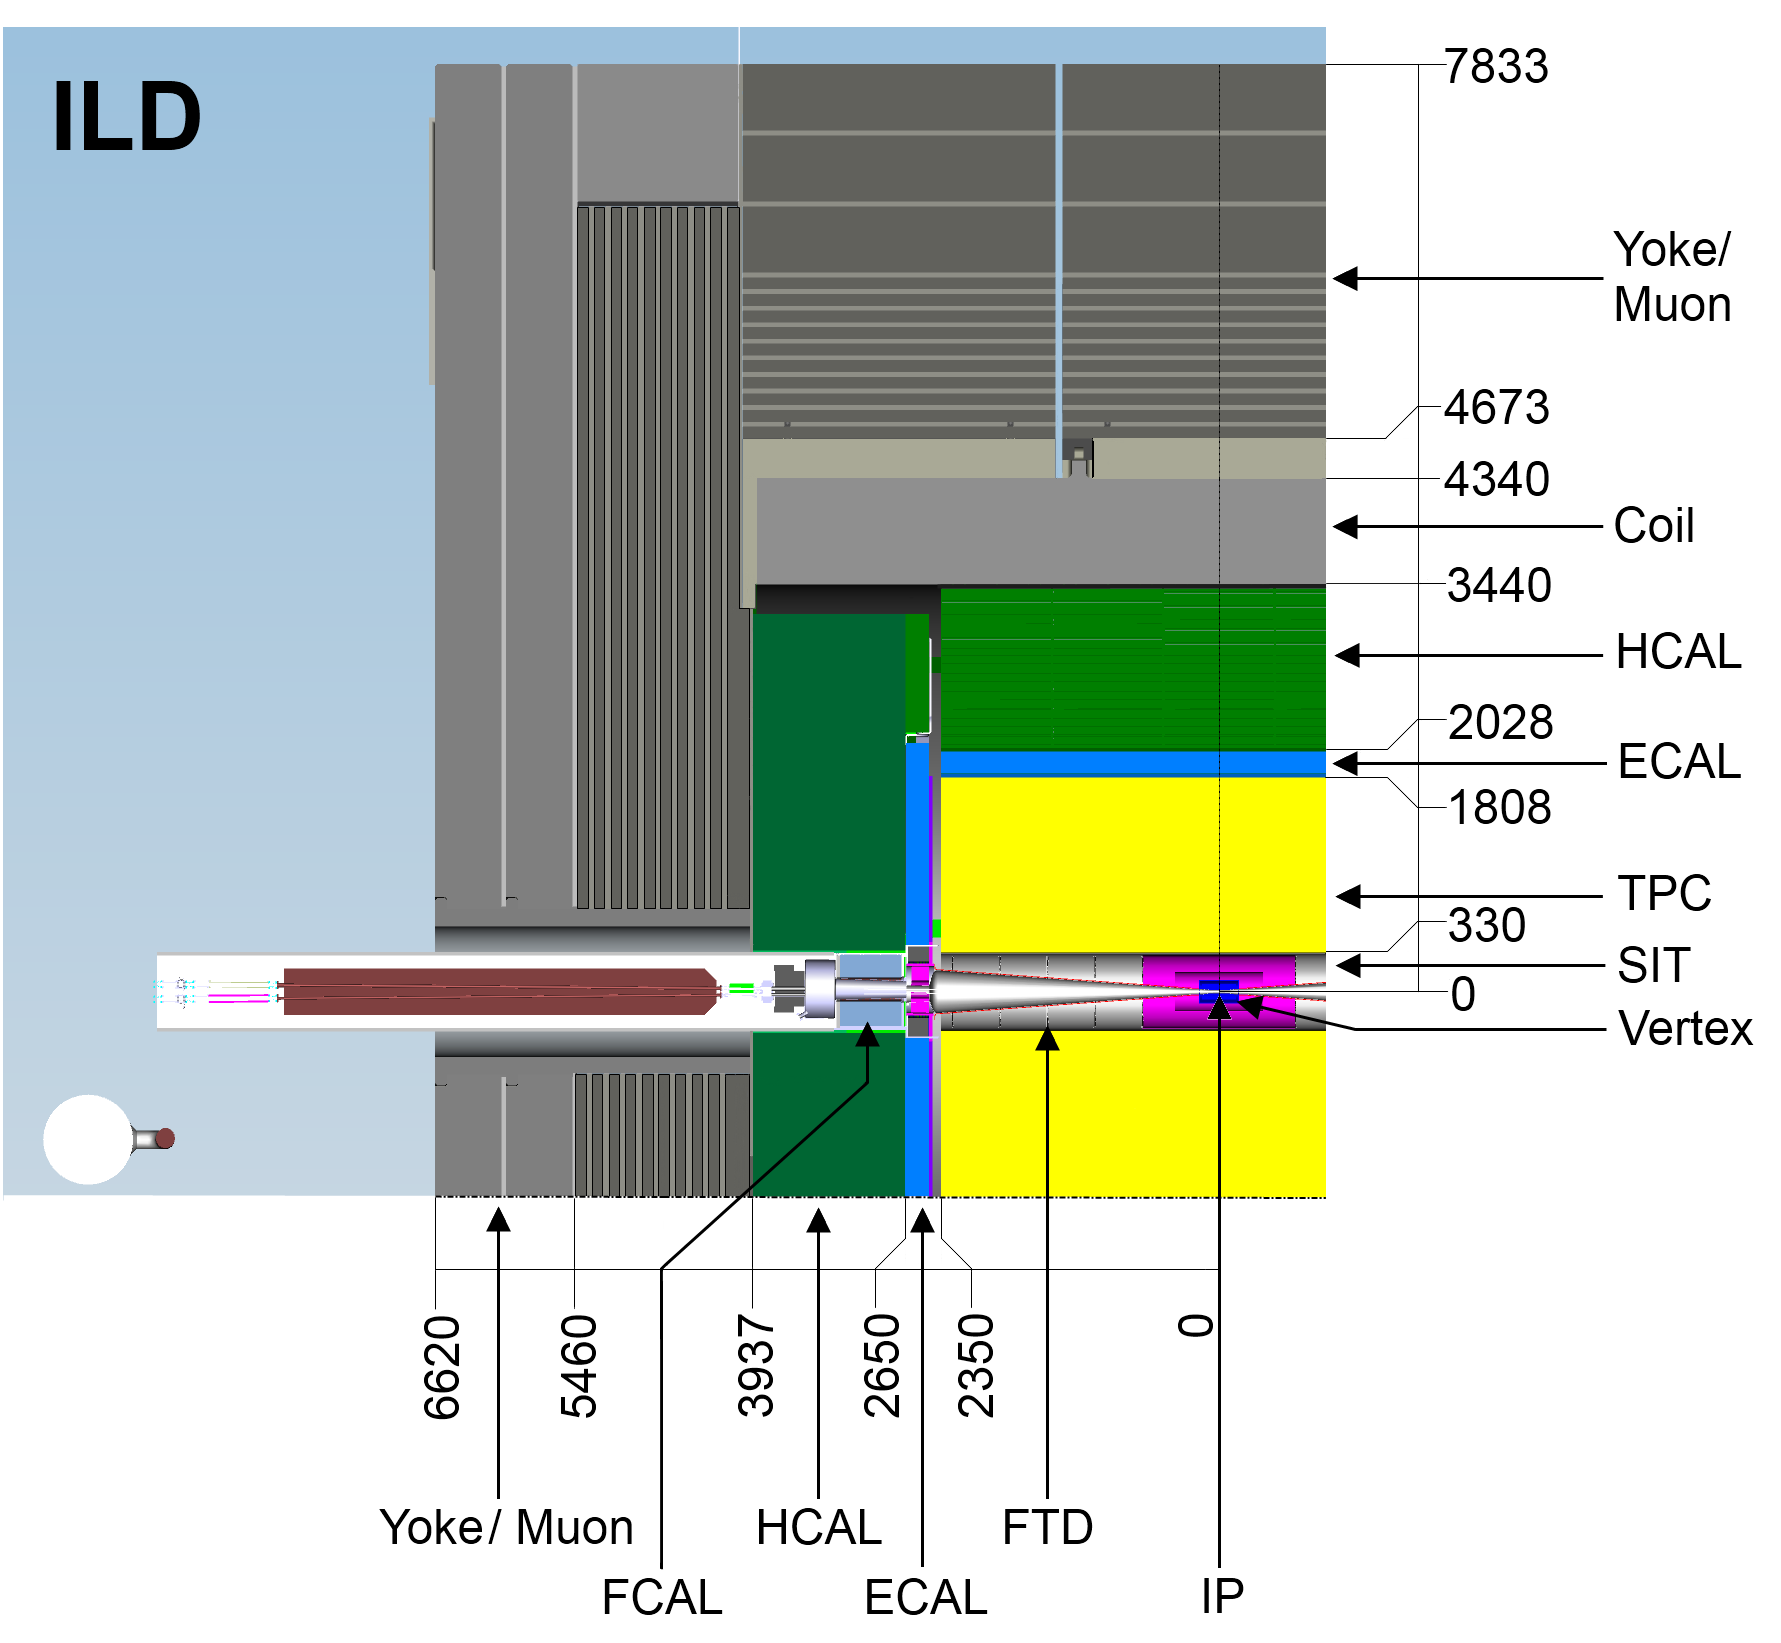
\includegraphics[width=0.8\hsize]{Detector/fig/ILD_quadrant_2.png}
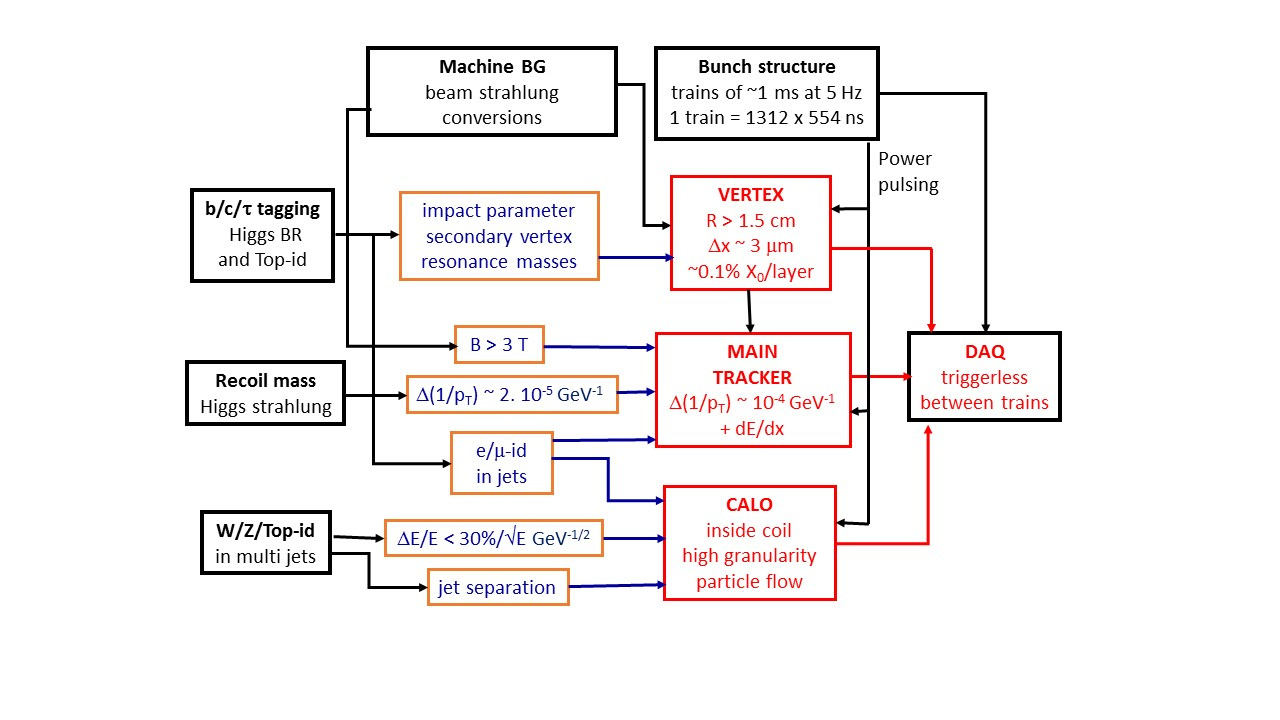
\includegraphics[width=1.0\hsize]{ILD/fig/ILD_specifications.jpg}
\caption{Interplay between ILC machine characteristics, physics requirements and detector specifications.}
\label{fig:ILD:specifications}
\end{figure}
%\textit{Detector performance aspects to be anticipated for higher energies}


\section{Optimizing ILD}

The baseline ILD layout of the DBD~\cite{ild:bib:ilddbd} had intentionally large dimensions in order to maximize the tracking performance and the particle flow capabilities of the calorimeters. The main cost drivers of the DBD detector were the electromagnetic calorimeter and the coil/yoke system, for which specific options are considered to reduce their costs (chapters 6.4 and 9). In the past years a re-optimization process of the detector global dimensions has been launched to identify an optimal point in the cost-performance space.

In a first step, a parametric study \cite{Ref:bib:TPCOPT} of the dependence of cost and performance as function of the outer radius and length of the main tracker (the TPC in ILD) has been performed. 
A simple model has been constructed, based on the cost estimate published as part of the ILD DBD~\cite{ild:bib:ilddbd}. In this model the cost of each subdetector is scaled as a function of the size based on simple scaling laws. Sensitive detector elements like Silicon planes are scaled with the total area, while mechanical elements - for example, the absorber in a calorimeter - scale with the volume. The reference is always the DBD cost estimate. To study the effect of changing the TPC radius and length, all other dimensions outside of the TPC are tied to the TPC radius and TPC length. Clearances between detectors are kept constant, and do not scale. In this way, an overall cost scaling of the ILD detector can be computed. Comparison with the more detailed updated costing presented in chapter 9 shows that this parametric scaling if correct at the level of 20-30\%. 

The performance of the detector is measured by a combined performance estimator, based on a few observables mostly from Higgs physics. Essentially, these are the tracking performance (momentum resolution and impact parameter resolution), the Higgs mass precision (with and without beam-strahlung background), the inverse of the significance of b-tagging, and the minimum transverse momentum to reach the last layer of the vertex detector. All numbers are normalised to the performance of the DBD detector. For a more complete description of the method and the definitions, see \cite{Ref:bib:TPCOPT}. 

Two types of iso-curves are then defined in the space opened by the TPC radius and length: Equal performance, and equal cost. In figure ~\ref{fig:ILD:aspect_ratio} iso-cost and iso-performance curves are shown. The three red lines correspond to costs relative to the DBD of (from top to bottom) 100\%, 90\% and 80\%. The blue lines indicate equal-performance lines. From the plot it can be seen that the dependence of the cost on the detector radius is steeper than on the length, while the performance scales roughly the same for both. This shows that targeting a given cost reduction maintains a higher performance when reducing the radius while keeping the overall length unchanged, instead of keeping the aspect ratio r/z unchanged.  

\begin{figure}[t!]
\centering
%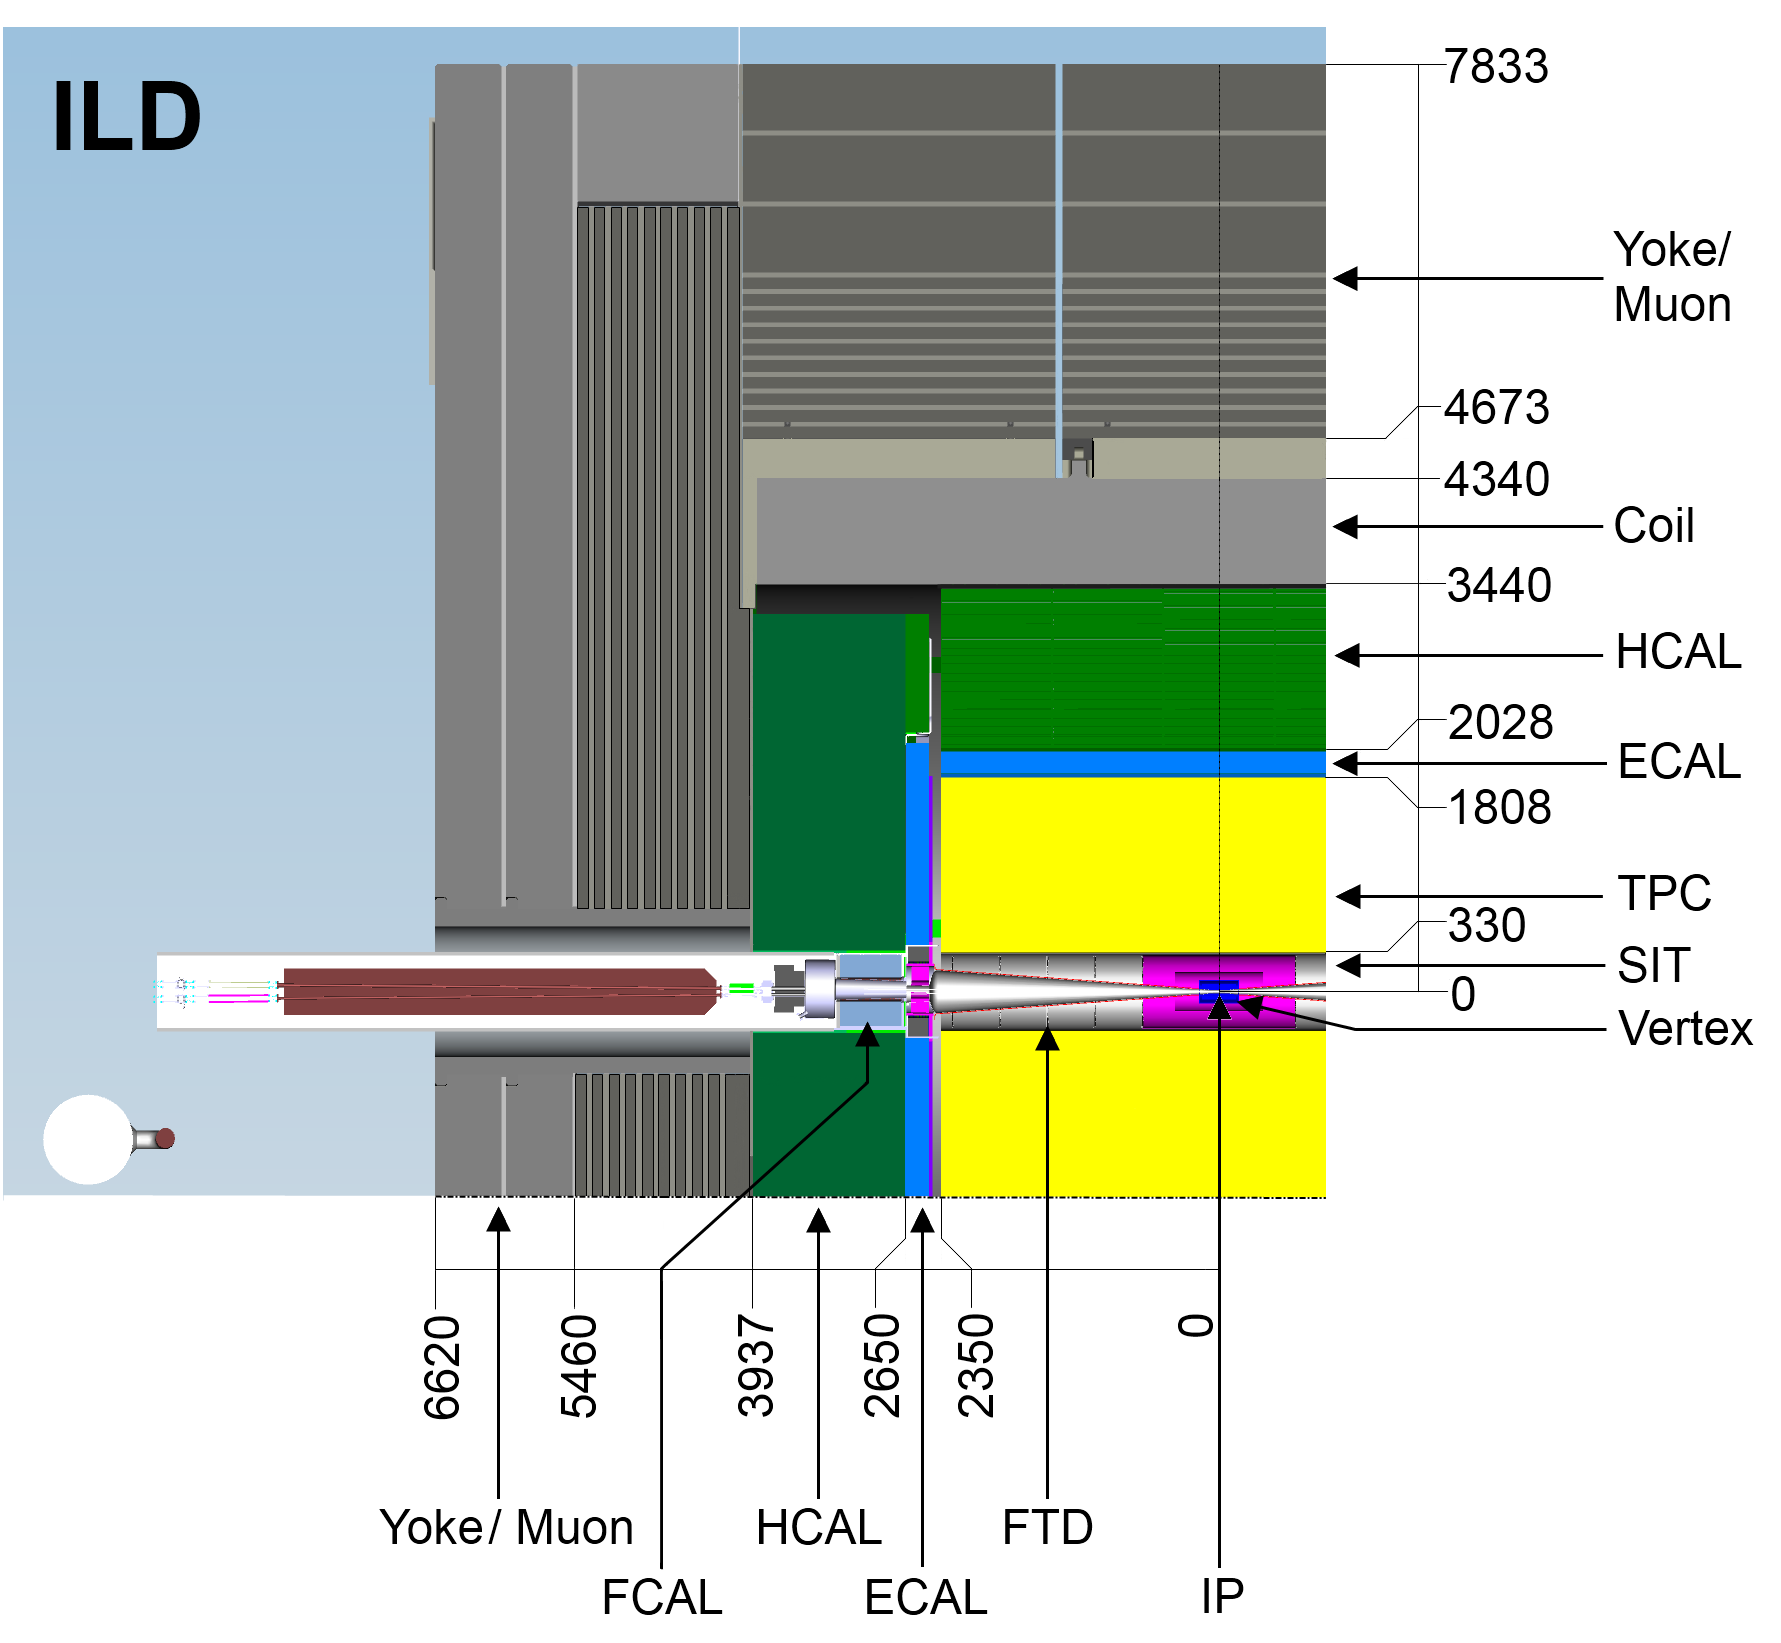
\includegraphics[width=0.8\hsize]{Detector/fig/ILD_quadrant_2.png}
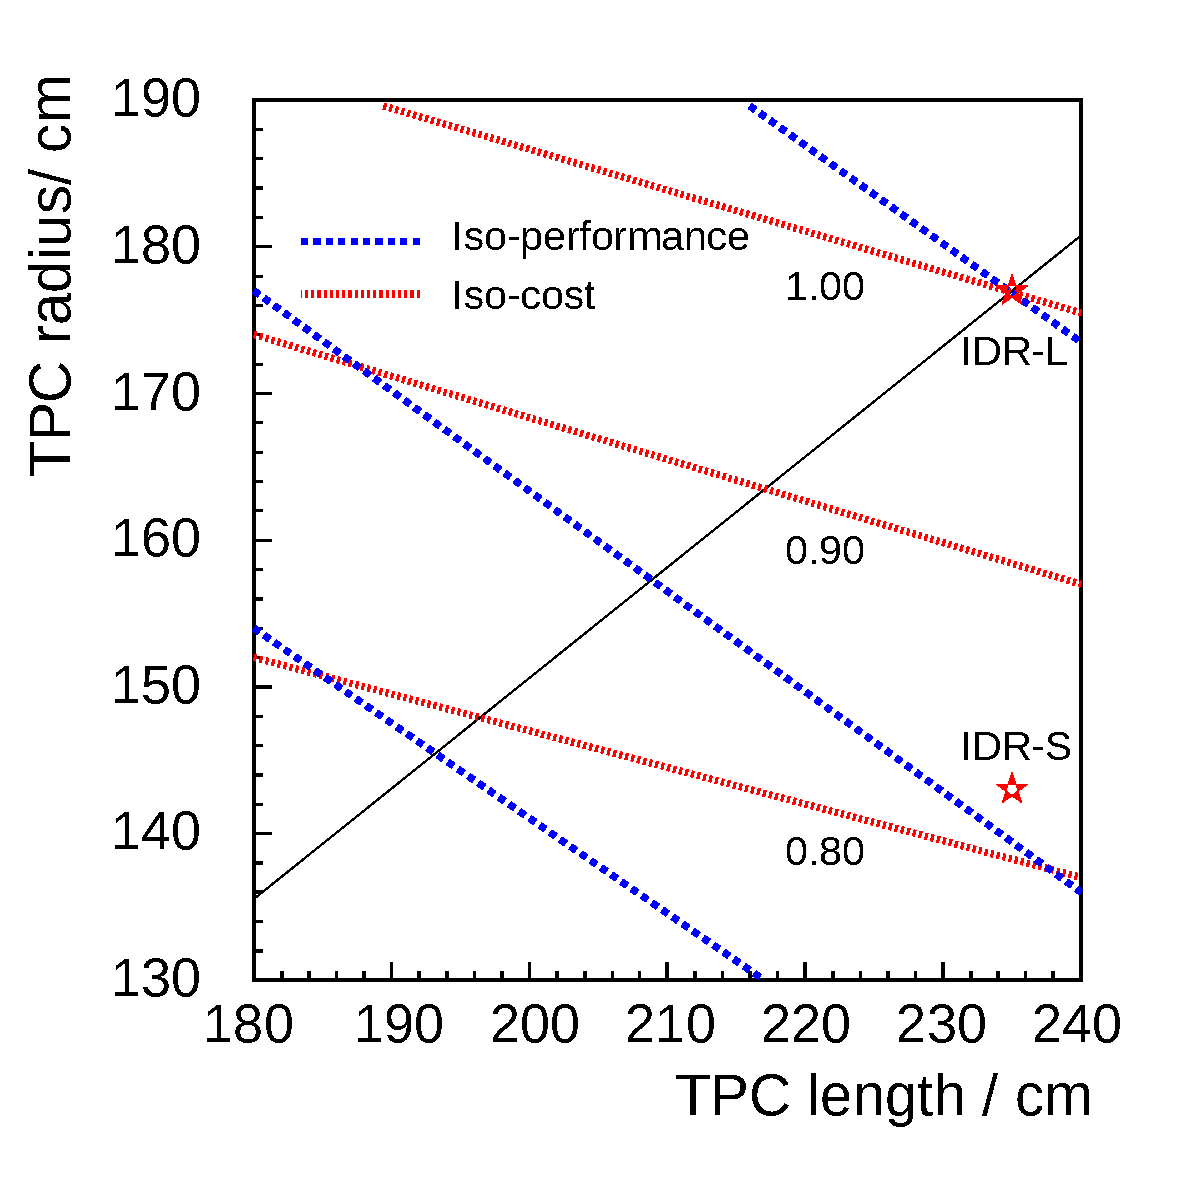
\includegraphics[width=0.5\hsize]{ILD/fig/aspect_ratio.pdf}
\caption{Iso-performance and iso-cost curves resulting from a parametric evaluation of the ILD detector in the tracker radius-length parameter space. The stars indicate the location of the different ILD models in this parameter space. The black diagonal line indicates dimension changes at a constant r/z aspect ratio.}
\label{fig:ILD:aspect_ratio}
\end{figure}

Based on this study, detector models with different sizes were defined with the following guidelines:

\begin{itemize}
    
\item The number of detector models is limited to two to maintain simulations and analyses at a manageable level.

\item One of the models ("IDR-L") has dimensions similar to those of the DBD model, in order to have a well understood reference in the studies. The only changes compared to the DBD are associated to the collider parameter evolution (e.g. the new L* optics, see chapter 3), and to better understanding of the subdetector technology constraints. This resulted in small changes to the TPC outer radius and length. 

\item The second model ("IDR-S") has a reduced outer radius of the main tracker while keeping its length unchanged. The smaller radius has to be far enough from the IDR-L radius to provide a significant lever-arm for the comparison. The chosen value is equal to that of the new CLIC detector model CLICdp~\cite{Arominski:2018uuz}, half way of the even smaller radius of the SiD detector~\cite{ild:bib:ilddbd}. With this choice IDR-S has similar outer tracker dimensions to CLICdp for both radius and length. This offers the possibility to compare the performance of the TPC option to the all-silicon option favored by CLICdp. 

\item All other components of IDR-S are similar to IDR-L. The inner tracking and very forward detectors are identical. The calorimeter depths and cell sizes are also kept unchanged, and the number of cells is reduced only as function of the calorimeter radii. All external systems such as coil, yoke and endcaps have their radial dimensions reduced accordingly.

\item In order to compensate for the smaller tracking lever-arm the nominal magnetic field of IDR-S is increased from 3.5\,T to 4\,T.

\end{itemize}

\begin{figure}[t!]
\centering
%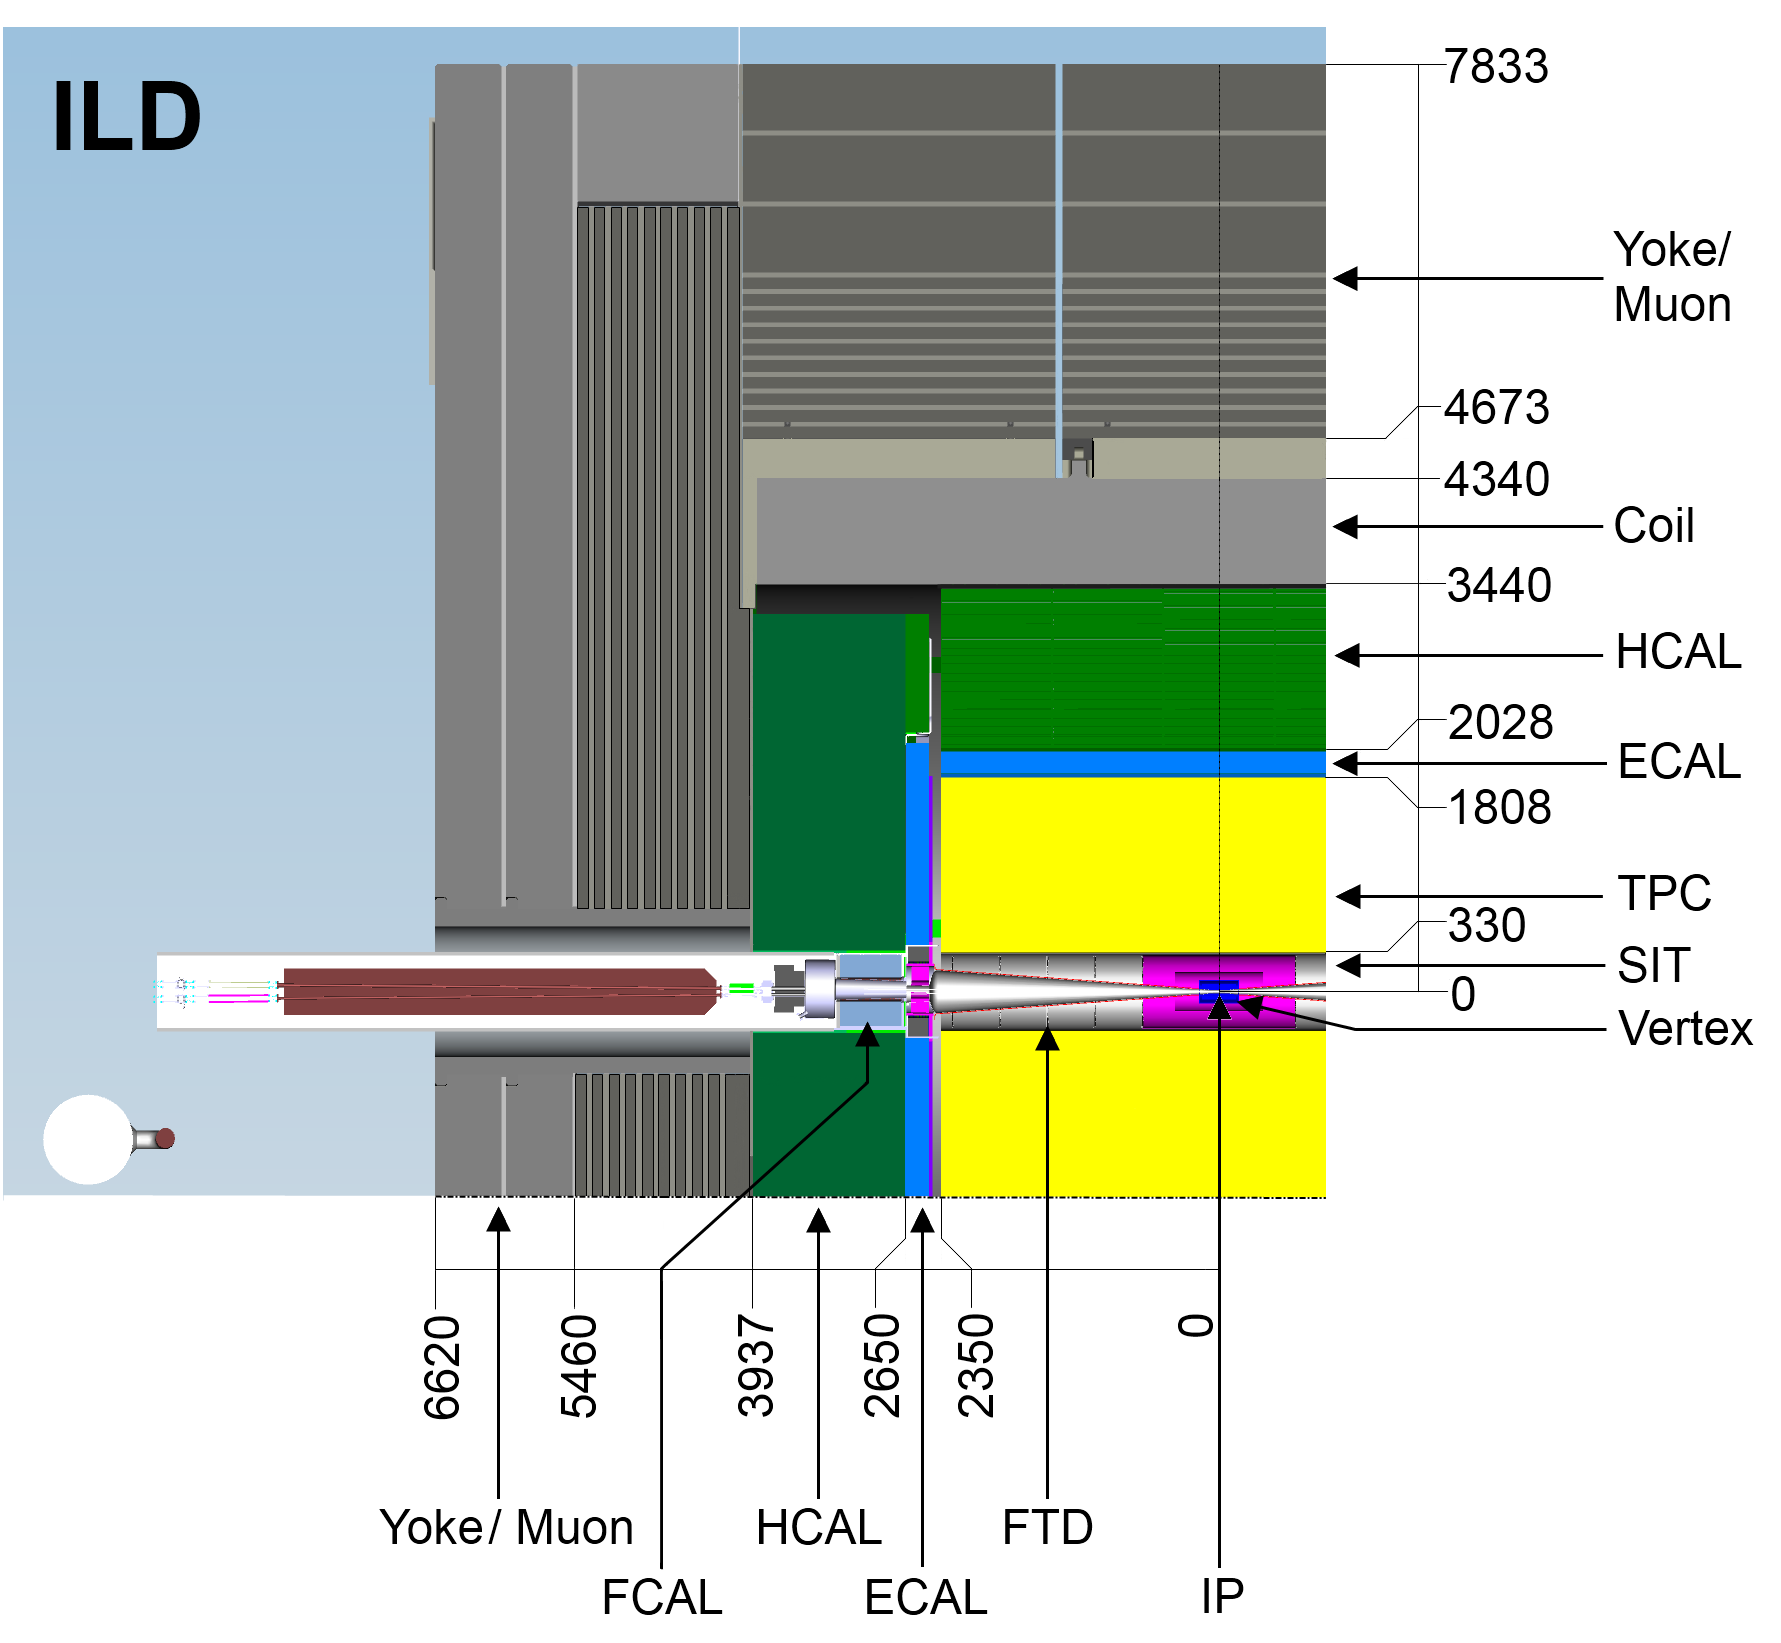
\includegraphics[width=0.8\hsize]{Detector/fig/ILD_quadrant_2.png}
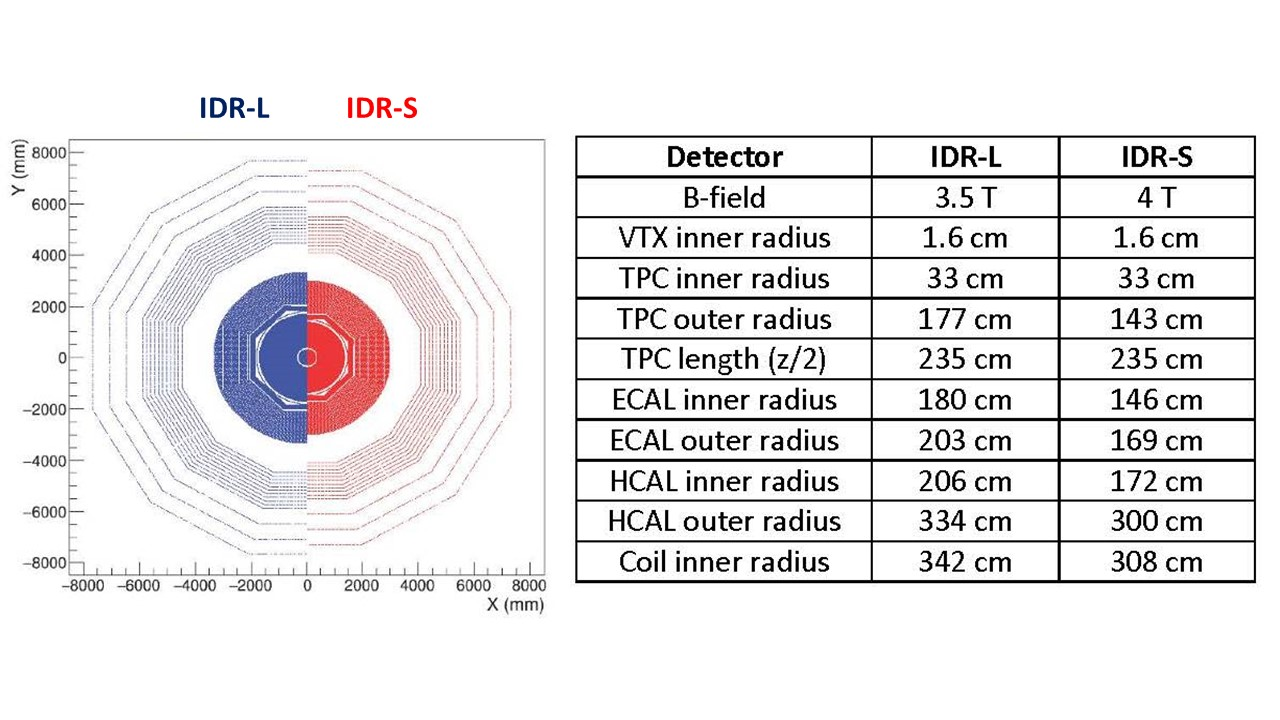
\includegraphics[width=1.0\hsize]{ILD/fig/ILD_small-large.jpg}
\caption{The large ("IDR-L") and small ("IDR-S") models used for the ILD optimization: R-$\phi$ view (left) and main subdetector dimensions (right).}
\label{fig:ILD:sizes}
\end{figure}

The resulting IDR-L and IDR-S dimensions are summarised in figure ~\ref{fig:ILD:sizes}. Both models were used for detailed simulations of physics benchmark samples. The simulation framework is described in chapter~\ref{chap:modelling}. The detector and physics performance of both models are compared in chapter~\ref{chap:performance} and their costing estimated in chapter~\ref{chap:costing}. \vfill


	